\chapter{Elementary Quantum Physics}
\thispagestyle{fancy}
\begin{multicols}{2}
Wien's Displacement Law
\begin{align}
\lambda_{MAX}T=2.898 \times 10^{-3}m*K
\end{align}
Total Power Stefan-Boltzmann Law
\begin{align}
R(T)= \int_{0}^{\infty}I(\lambda,T)d\lambda = \epsilon \sigma T^4 \\
\epsilon = \textrm{emmisivity (unitless)} \\
\sigma = 5.67 \times 10^{-8}\frac{w}{m^2k^4}
\end{align}
Max Planck's Radiation Law:
\begin{align}
I(\lambda,T)=\frac{2\pi c^2h}{\lambda^5}\frac{1}{e^{hc/\lambda kT}-1}
\end{align}
The kinetic energy of an emitted photoelectron is (Where $\phi =$ binding energy of electron to metal surface or the work function)
\begin{align}
KE &= hv- \phi \\
E_{photon} &= KE_{electron} + \phi \\
KE_{electrons} &=0 \textrm{ (at threshold)}
\end{align}

Ruthford Scattering Formula:Any particle hitting an area $\sigma$ around the nucleus will be scattered through an angle of $\theta$ or greater.
\begin{align}
b &= (r_{min}/2) \cot (\theta /2) \\
r_{min} &= \frac{Z_1Z_2e^2}{4 \pi \epsilon_0 K} \\
\sigma &= \pi b^2 = \textrm{ cross sectional area } \\
\frac{e^2}{4\pi\epsilon_0} &= 1.44 \times 10^{-9} \textrm{eV$\cdot$m}
\end{align}
A common unit of $\sigma$ is one barn.
\begin{align}
\textrm{barn (unit)} &= 10^{-28} m^2 = 100 fm^2 \\
\frac{ \textrm{\# atoms} }{ \textrm{area} } &= \frac{ \textrm{atoms} }{ \textrm{volume} } \times \textrm{thickness}
\end{align}
\begin{align}
n &= \bigg(N_A\frac{atoms}{mole}\bigg)\bigg(\frac{1}{A}\frac{mole}{gm}\bigg)\bigg(\rho \frac{gm}{cm^3}\bigg) \\ &= \frac{\rho N_A}{A}
\end{align}

The Compton effect describes the photon wavelength $\lambda'$ after a photon of wavelength $\lambda$ scatters off an electron.
\begin{align}
\lambda' &= \lambda + \frac{h}{m_ec}(1-cos(\theta)) 
\end{align}
The Compton wavelength of an electron is 
\begin{align}
\lambda_e = \frac{h}{m_ec}= 2.426 \times 10^{-12}m
\end{align}
Heisenberg Uncertainty relation
\begin{align}
	\Delta x \Delta p_x \geq \frac{1}{2}\hbar
\end{align}
The de Broglie wavelength is defined as
\begin{align}
\lambda &= \frac{h}{p} = \frac{h}{mv\gamma} = \frac{h}{mv}\sqrt{1-\frac{v^2}{c^2}} \\ &= \frac{hc}{\sqrt{K_E^2 + 2K_EE_0}}
\end{align}
Rutherford Scattering.
\begin{align}
K &=\frac{1}{4\pi \epsilon_0}\frac{Z_1Z_2e^2}{R_{min}} \\ R_{min} &=\frac{1}{4\pi \epsilon_0}\frac{Z_1Z_2e^2}{K}
\end{align}
Z's are the atomic masses of the particles within the interaction and $R_{min}$ is the minimum distance they reach (from center to center), and e is 
\begin{align}
e &=1.602177\times 10^{-19} C \\
\epsilon &\approx 8.854 \times 10^{-12} F/m
\end{align}
The Rutherford Scattering Formula
\begin{align}
N(\theta) &= \frac{N_int}{16r^2}(R_{min})^2\frac{1}{\sin^4(\theta/2)}
\end{align}
Centripetal force due to coulomb attraction
\begin{align}
\frac{1}{4\pi \epsilon_0} \frac{e^2}{r^2} &=ma_c=m\frac{v^2}{r}\\ &\implies v^2=\frac{1}{4\pi \epsilon_0}\frac{e^2}{mr} \\
&\implies r = 4\pi\epsilon_0\frac{n^2\hbar^2}{me^2}
\end{align}
Energy levels 
\begin{align}
E&=KE+PE \\&= -\frac{1}{2}\frac{e^2}{4\pi \epsilon_0r}\\ &\implies E =\frac{-E_0}{n^2}, \\
&\textrm{where $E_0=\alpha^2mc^2/2 = 13.6$ eV.}
\end{align}
Energy of emitted radiation
\begin{align}
E&=E_n-E_m \\ &= E_0\bigg(\frac{1}{m^2}-\frac{1}{n^2}\bigg)
\end{align}
\begin{note}
	Using the Planck formula in the above equation leads to the Rydberg formula.
\end{note}

The Rydberg formula: Wavelength of the spectral lines in Hydrogen:
\begin{align}
\frac{1}{\lambda} &=R_H \bigg(\frac{1}{n_f^2}-\frac{1}{n_i^2} \bigg) \\
n \in \mathbb{N} &= 1,2,3,4,5,\dots 
\end{align}

\begin{note}
	ZnS (Zinc Sulfide) emits a faint flash of light when struck by an $\alpha -$ray.
\end{note}
L quantized
\begin{align}
L=mvr=n\hbar
\end{align}
Stationary state orbits
\begin{align}
r &=a_0n^2 \\
a_0 &= \textrm{Bohr Radius}
\end{align}
Stationary state energies
\begin{align}
E_n &=-Z^2\frac{E_0}{n^2}
\end{align}
Uncertainty relation of energy and the measurement of time.
\begin{align}
\Delta E \cdot \Delta t \geq \frac{1}{2} \hbar
\end{align}
\end{multicols}
Bragg's Law: When scattering off of crystal structures, the wavelengths will peak at specific angles determined by the diagrams below
\begin{align}
n\lambda &=2d\sin(\theta)=2d\cos(\alpha) = 2D\sin(\alpha)\cos(\alpha) =D\sin(2\alpha) = D\sin(\phi)\\
d &= Dsin(\alpha) \\
\phi &= 2 \alpha \\
\theta &= 90^\circ - \alpha
\end{align} 
\begin{center}
	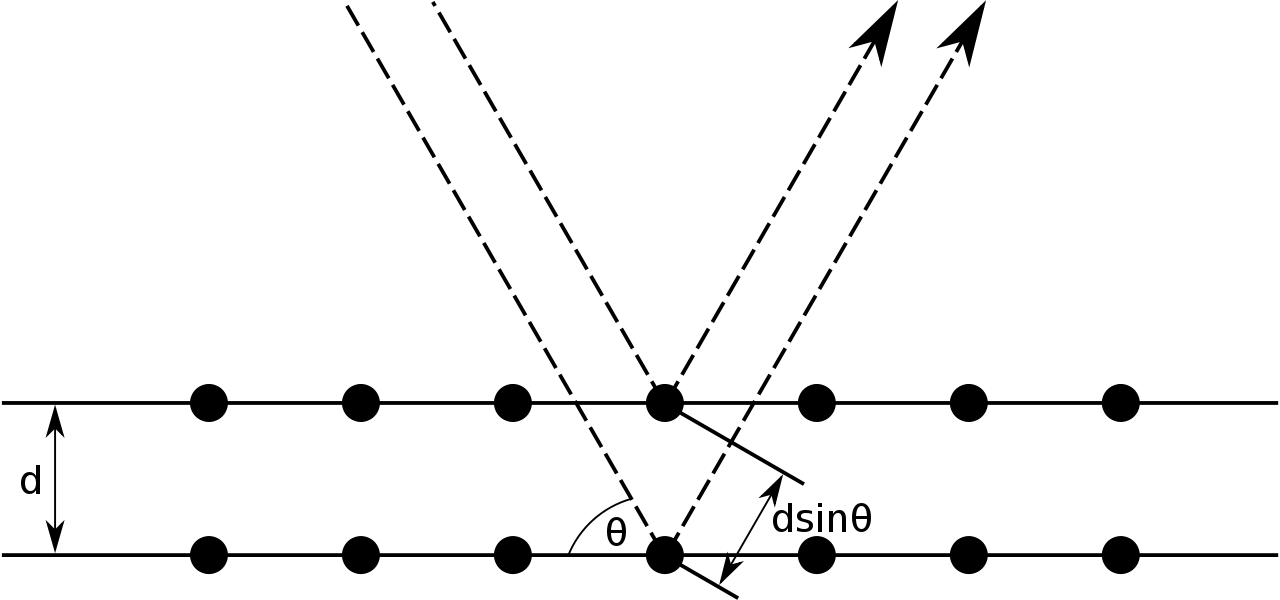
\includegraphics[scale=0.2]{./Images/Diagrams/1280px-BraggPlaneDiffraction.png} 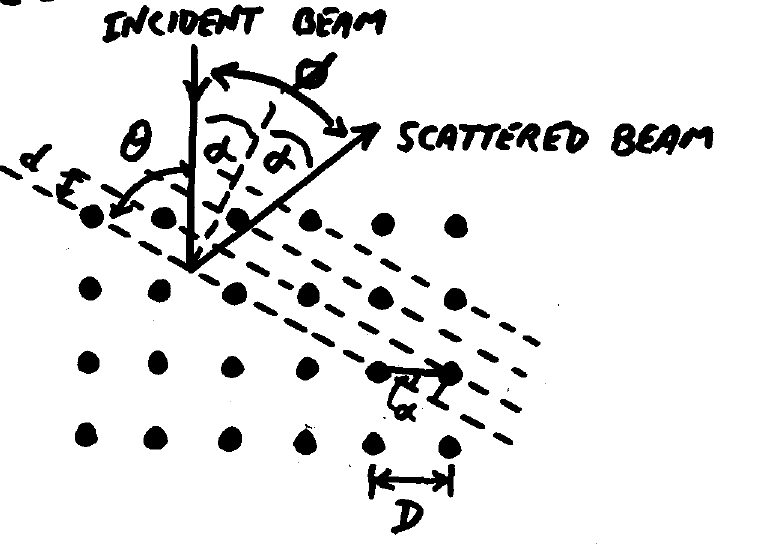
\includegraphics[scale=0.25]{./Images/Diagrams/crystalscattering.png}
\end{center}





The potential the electron moves in
\begin{align}
V(r)=\frac{-e^2}{(4\pi \epsilon_0r)}
\end{align}
The angular momentum of an electron in the atom
\begin{align}
L=mvr=\hbar\sqrt{\ell(\ell+1)} \\
L_z=m_\ell\hbar 
\end{align}
An electron orbiting around a nucleus has magnetic moment $\vec{\mu}$
\begin{align}
\vec{\mu}&=IA\hat{n}=\frac{-e}{(2\pi r/v)}(\pi r^2)\hat{n}=\frac{-erv}{2}\hat{n}=\frac{-e}{2m}\vec{L} \\
\mu_z&=\frac{-e}{2m}L_z=\frac{-e}{2m}m_l\hbar=-m_\ell\mu_B 
\end{align}
In an external magnetic field, $B$, the
magnetic dipole feels a torque $\vec{\tau}$ and has a potential energy $U_B$
\begin{align}
\vec{\tau}&=\vec{\mu}\times \vec{B} \\
V_B&=-\vec{\mu}\cdot \vec{B} = \frac{-e}{2m}\vec{L} \cdot \vec{B} \implies V_{Bz}= \mu_B m_\ell B_z
\end{align}
